\section{Method}\label{sec:method}

Being a system distributed across distinct computing platforms (a general
purpose computer; a network of microcontrollers), and software elements
serving a variety of purposes (server and client instances for transmission
and reception of networked audio and control data, plus a digital
signal processing algorithm), it is important to consider each of these
elements in detail.
In the sections to follow, these elements are described;
finally an overview of the devised system is provided.

\subsection{The Networked Audio Server}\label{subsec:the-networked-audio-server}

TCP is, as described in \secref{subsubsec:protocols-systems}, a
connection-based, one-to-one protocol, so the JackTrip connection model enforces
a sort of pseudo-connectionfulness on the otherwise connectionless UDP.\
The result is a system which permits only unicast UDP transmission, and, for
multiple clients, must send a duplicate of the outgoing stream of audio
datagrams to each connected client.
A JackTrip server creates a sender and a receiver task for each client that
connects~\citep{caceres_jacktrip_2010};
notionally this entails, should enough clients connect, exhaustion of all
available network bandwidth;
as such, a unicast system does not meet the requirement of scalability as
described in \secref{subsec:distributed-audio-systems}.

%With a view to exploiting the UDP multicast capabilities of NetJACK, initial
%efforts centred on an attempt to create a NetJACK client for the Teensy
%platform.
%\begin{inparaenum}[1)]
%    \item NetJACK was created as a general-purpose system, with functionality
%    beyond the requirements of the proposed implementation;
%    \item JACK has not served as a truly cross-platform audio host for a
%    number of years; although \texttt{jackd} runs on Mac OS X systems, not
%    since OS X 10.14 has JACK been compatible with Mac's CoreAudio
%    API, thus any server implementation based upon NetJACK would not be
%    operable on a modern Mac operating system.\footnote{
%        For more information, see Stéphane Letz's proposed design for a
%        successor to the defunct CoreAudio/JACK bridge
%        \url{https://github.com/jackaudio/jack-router/blob/main/macOS/docs/JackRouter-AudioServerPlugin.md}
%        (accessed 04/01/2024).
%    }
%\end{inparaenum}

%Of course, being tied to JACK as its audio host, the latter rationale applies
%also to the JackTrip-based approach.
%This being the case, attention was turned to the design of a bespoke multicast
%networked audio system.

A multicast NetJACK server was considered, but creating a client implementation
on what is essentially a bare-metal platform in the shape of the Teensy, was not
practical.
Further, due to a break in compatibility with Mac OS X systems, JACK-based
approaches are not truly cross-platform.\footnote{
    A successor to the defunct CoreAudio/JACK bridge has been proposed but
    remains unrealised:
    \url{https://github.com/jackaudio/jack-router/blob/main/macOS/docs/JackRouter-AudioServerPlugin.md}.
    This issue of course also affects the viability of the JackTrip-based
    approach.
}
Prioritising simplicity, in the form of an audio server having minimal
dependencies and a very specific task to achieve, attention was turned to the
design of a bespoke multicast networked audio server.

\subsubsection{Designing a Networked Audio Protocol}\label{subsubsec:designing-a-protocol}

Dependent on the intended application, and if assumptions can be made about
matters such as sampling rate and bit resolution, a \textit{no-protocol}
approach, such as described by Lopez-Lezcano~\citep{lopez-lezcano_jack_2012},
may be a viable one.
To make the new system somewhat flexible and future-proof, however, a simple
packet header was devised.
Its structure is given in \lstref{listing:packet-header}.

\begin{codelisting}{
    Packet header structure,
    label=listing:packet-header,
    minted language=cpp,
    minted style=xcode,
    float=ht
}
    struct PacketHeader {
        uint16_t SeqNumber;
        uint8_t BufferSize;
        uint8_t SamplingRate;
        uint8_t BitResolution;
        uint8_t NumChannels;
    };
\end{codelisting}

The resulting six-byte header comprises a two-byte (unsigned 16-bit integer)
packet sequence number, to be incremented by the sender, plus four further bytes
describing the structure of the audio data in the packet.
Commonly-encountered sampling rates, and buffer sizes greater than 255, cannot
be represented by unsigned eight-bit integers, so
these are backed up by enumerations inspired by those used by JackTrip\footnote{
    \url{https://github.com/jacktrip/jacktrip/blob/v1.6.8/src/AudioInterface.h\#L56}
}:

%\begin{multicodelisting}{Supporting enumerations for packet metadata,
%    label=ls:packet-enums,
%    top=0pt,
%    bottom=0pt
%}
%    \begin{tcbraster}[threecolraster]
%        \begin{multicodesublisting}[minted language=cpp, minted style=xcode]
%            enum BufferSizeT {
%                BUF8 = 3,
%                BUF16,
%                BUF32,
%                BUF64,
%                BUF128,
%                BUF256,
%                BUF512,
%                BUF1024,
%                BUF2048,
%                BUF4096
%            };
%        \end{multicodesublisting}
%        \begin{multicodesublisting}[minted language=cpp, minted style=xcode]
%            enum BitResolutionT {
%                BIT8 = 1,
%                BIT16,
%                BIT24,
%                BIT32
%            };
%        \end{multicodesublisting}
%        \begin{multicodesublisting}[minted language=cpp, minted style=xcode]
%            enum SamplingRateT {
%                SR22,
%                SR32,
%                SR44,
%                SR48,
%                SR88,
%                SR96,
%                SR192
%            };
%        \end{multicodesublisting}
%    \end{tcbraster}
%\end{multicodelisting}
\noindent
A buffer size of 16 is represented by \mintinline{cpp}{BufferSizeT::BUF16},
which is assigned the number 4, the appropriate power of two to use in
converting between the enumeration and the number with which it corresponds.
Similarly, a bit resolution of 16 is associated with
\mintinline{cpp}{BitResolutionT::BIT16}, which takes the value 2, the number of
bytes in a 16-bit integer.

For well-formed packets, \mintinline{cpp}{BufferSize} could in fact
be inferred from the size of the packet (minus its header), divided by
\mintinline{cpp}{NumChannels} and \mintinline{cpp}{BitResolution}, the latter
treated as the number of bytes per sample (as per the enumeration value).
To permit scope for the detection of malformed packets, however, the expense
of an additional byte in the header was deemed a reasonable one.
The sequence number will wrap around every 65,536 packets, and is intended as
a means for a recipient to identify the occurrence of packet loss.

\subsubsection{Server Design}

\begin{figure}[ht]
    \centering
    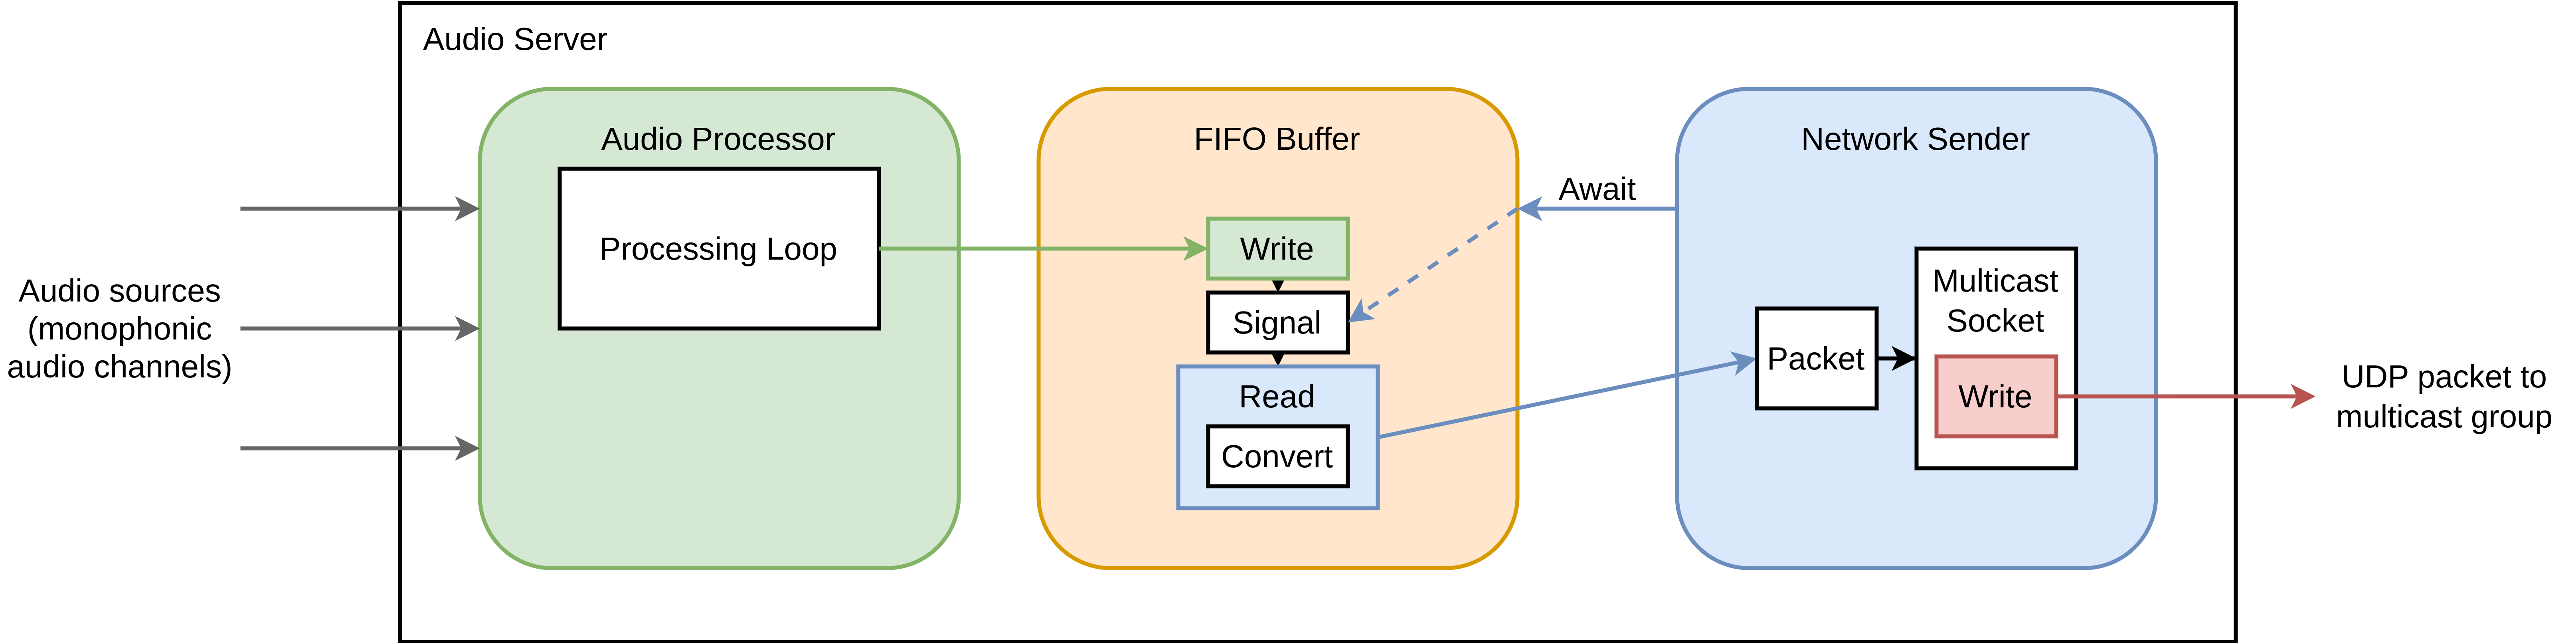
\includegraphics[width=\textwidth]{figures/audio-server}
    \caption{Overview of operation of the networked audio server.
    The network sender awaits notification of readiness to read samples from a
    first-in-first-out buffer of audio samples.
    The audio processor receives audio channels from a multichannel source
        (e.g. a DAW); at each iteration of its processing loop, it writes samples
        to the FIFO; upon write-completion, the FIFO sends a signal to the network
        sender that a block of samples is ready.
        Samples are converted to the appropriate format, and bundled into a UDP
        packet which is then written to the network.}
    \label{fig:audio-server}
\end{figure}

The networked audio server was written in C++ using utility classes provided by
the JUCE framework for the development of audio applications.\footnote{
    JUCE 7.0.5 \url{https://github.com/juce-framework/JUCE}
}
The server is encapsulated as a class called \texttt{NetAudioServer},
which can be incorporated into any JUCE-based audio application;
initial development was conducted on a basic console application, and later work
targeted a DAW plugin comprising a consolidated audio server and wave field
synthesis controller.

The \texttt{NetAudioServer} instance expects to receive blocks of
multichannel audio from an audio application's main processing loop.
It sets up network \textit{sender} and \textit{receiver} execution threads, and
assigns a network socket to each; a socket is essentially a numerical identifier
for an \textit{``endpoint for [network] communication''}
~\citep{kerrisk_socket2_2023} to which a type \textemdash{}
\texttt{SOCK\_STREAM} for TCP on \texttt{SOCK\_DGRAM} for UDP \textemdash{} can
be assigned.
To avoid potentially blocking the audio application's main processing thread
with networking operations, upon receiving an audio block the server writes it
to an intermediate buffer \textemdash{} a first-in-first-out (FIFO) structure
\textemdash{} and signals to the sender thread that a block is ready for
transmission.
The sender thread, which as been awaiting such a signal, then requests samples
from the FIFO; these are stored as contiguous channels of 32-bit floating point
samples and converted, when requested, to the bit resolution specified in a
packet header created when \texttt{NetAudioServer} is initialised.
Upon receiving the requested samples, the sender thread writes these to its
socket, which has been configured to connect to a UDP multicast group.

\lstref{listing:audio-packet} shows an example network capture of an outgoing
audio packet:

\codeinputlisting[float=h]
{text}
{listings/audio-packet.txt}
{Network capture: ethernet frame containing a UDP audio packet}
{audio-packet}

Bytes \texttt{0x0000} to \texttt{0x0029} comprise the ethernet, IPv4, and UDP
headers, including the destination address: at position \texttt{0x001e}, the
bytes \texttt{0xe004e004}, or \texttt{224.4.224.4}, a valid (and unassigned)
UDP multicast address from the second ad-hoc address block as specified in the
IANA multicast address assignment guidelines~\citep{meyer_iana_2010}.
The six subsequent bytes are the header inserted into the packet by
\texttt{NetAudioServer}.
In \lstref{listing:audio-packet} these are:
\begin{itemize}
    \item~\texttt{0xdf1c}: a sequence number (little-endian) of
    \numDec{7391};\footnote{Subscript 10 is employed here to indicate that we
    are dealing with a decimal number.}
    \item~\texttt{0x04}: buffer size \num{4} corresponding with
    \texttt{BUF16};
    \item~\texttt{0x02}: sampling rate \num{2} corresponding with
    \texttt{SR44};
    \item~\texttt{0x02}: bit resolution \num{2} corresponding with
    \texttt{BIT16};
    \item~\texttt{0x02}: \num{2} audio channels.
\end{itemize}

Audio data begins at byte \texttt{0x0030}.
Since the header indicates that there are two channels of 16-bit audio, and a
buffer size of 16 (samples, or rather frames of two channels worth of samples),
it is clear that the data for channel 1 encompasses the 32 bytes from
\texttt{0x0030} to \texttt{0x004f}, and channel 2 the remaining bytes.

Here, channel 1 is a test signal, a unit amplitude-increment unipolar sawtooth
wave, i.e.\ a signal whose amplitude starts at zero, and increments by 1 at each
sample until it reaches the maximum value that a signed 16-bit integer may take
\textemdash{} \numDec{32767} \textemdash{} at which point it wraps around to
zero and repeats.
This test signal serves two important purposes.
First, its impulse-like behaviour once every \num{32768} samples (roughly
\qty{.74}{\s} at a sampling rate of \qty{44.1}{\kHz}) is useful for taking basic
synchronicity measurements, e.g.\ involving connecting two clients' audio
outputs to an oscilloscope.
Second, this numerically-predictable signal served as a means to inspect the
integrity of the audio server algorithm, and to identify the appropriate
endianness for transmission.
Inspecting the first sixteen samples of the first audio channel
%(grouped
%by sample for legibility, see \lstref{listing:chan-1-samples}),
it is evident
that the amplitude values increment on a per-sample basis, and, since it is the
first byte that increases with each sample, that samples are transmitted little
endian.

%\codeinputlisting[float=h]
%{text}
%{listings/audio-packet-excerpt.txt}
%{Extracted samples from the transmitted unipolar sawtooth wave}
%{chan-1-samples}

The receiver thread polls its socket for traffic reaching the multicast group
from clients, and uses the presence of an incoming packet stream as proof that
a client is connected.

\paragraph{Transmission Considerations}\label{par:transmission-considerations}

Ethernet frames, and UDP datagrams by extension, are subject to size
limitations.
The maximum transmissible unit (MTU) of a transport medium is the limit on the
size of a packet that can be sent without fragmentation, i.e.\ without being
split into multiple sub-packets.
Two bytes are allocated to the `Total Length' field of the IPv4 header, which
suggests an MTU of $2^{16}-1=~$\num{65535} bytes;
in practice, however, the data link layer imposes a basic limit of \num{1500}
bytes on the payload of an ethernet
frame~\citep{schiavoni_alternatives_2013,ieee_ieee_2018}.

With the headers for the data link (Ethernet), network (IPv4), and transport
(UDP) layers accounted for, plus the audio header described above, in principle
\num{1452} bytes remain in each packet for audio data.
Assuming 16-bit resolution, and the transmission of one UDP packet per audio
buffer, data for up to 90 audio channels can be transmitted at a buffer size of
16 frames without fragmentation, or up to 45 channels at 32 frames.

\subsection{The Networked Audio Client}\label{subsec:networked-audio-client}

\begin{figure}[ht]
    \centering
    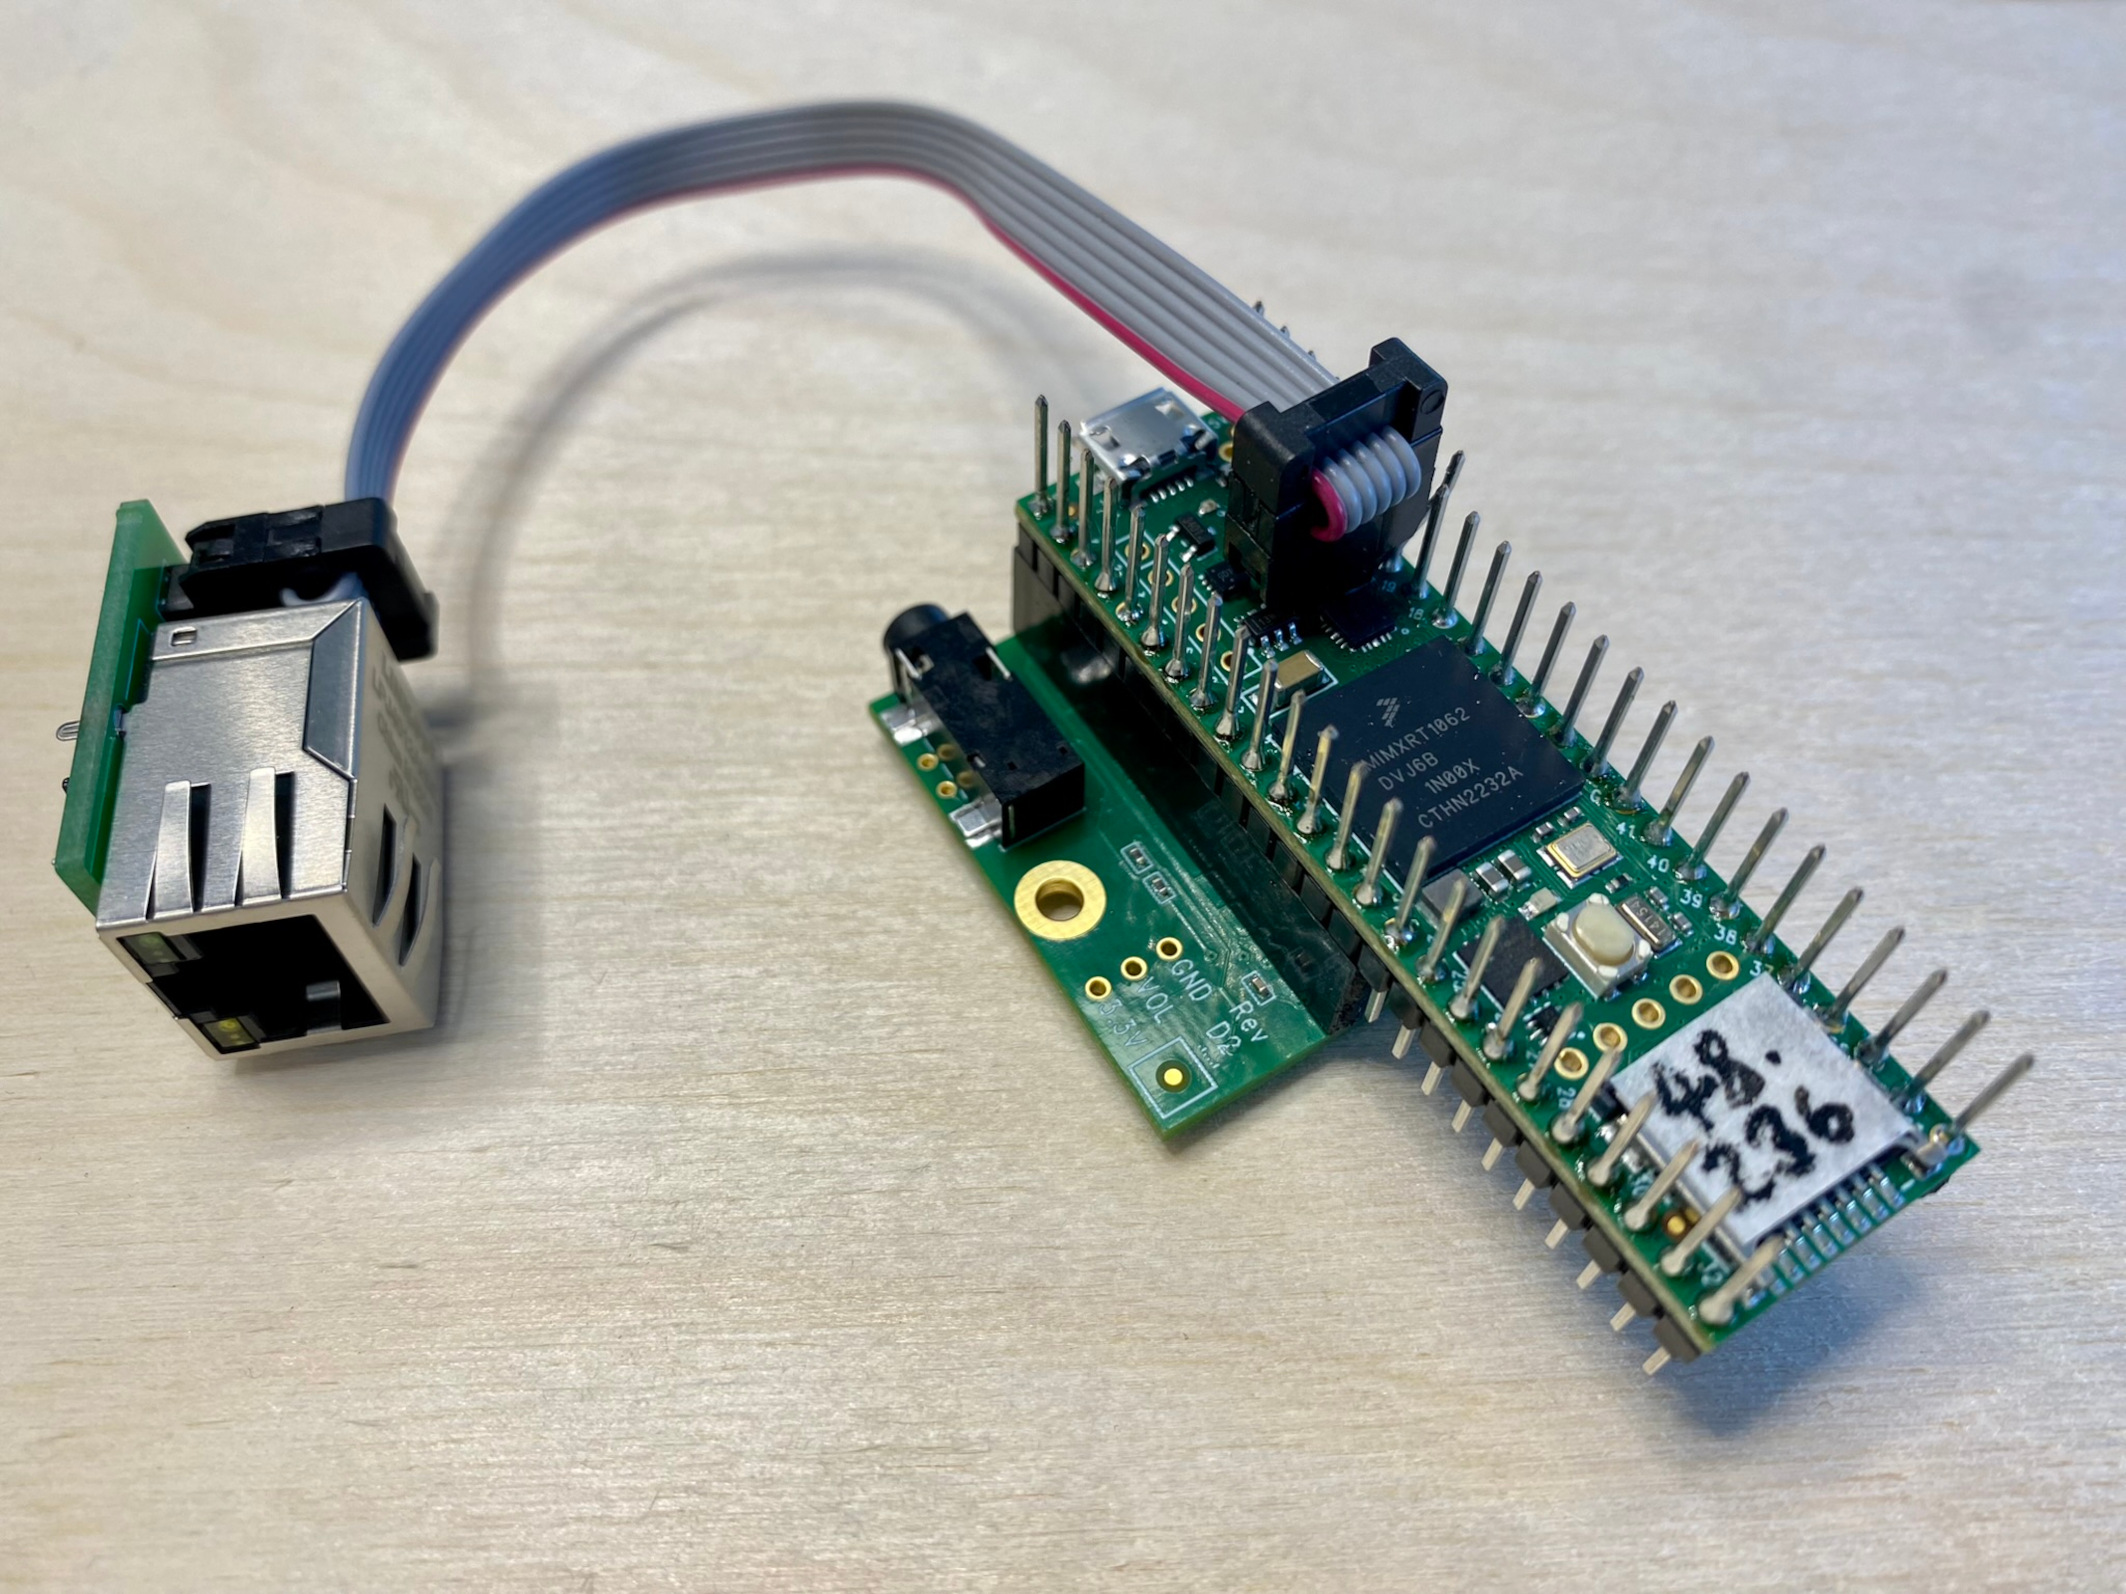
\includegraphics[width=.75\textwidth]{figures/module}
    \caption{A hardware module consisting of Teensy 4.1 microcontroller
        (labelled with the last two bytes of its serial number-derived IP address),
        connected via headers to an audio shield and via ribbon cable to an
        ethernet shield.}
    \label{fig:teensy}
\end{figure}
\noindent
Unlike the networked audio server, which runs on a general purpose computer and
has access to threads of execution, which it can use to conduct related but
separate tasks that rely on some central resource (the FIFO buffer alluded to
above), the client implementation is designed to operate on a microcontroller
platform that has no operating system, and no native notion of threads\footnote{
    There is in fact a non-core library, \textit{TeensyThreads}, that provides
    thread-like functionality. It was experimented with during development,
    but found to be incompatible with the interrupt-driven nature of the
    Teensy audio and networking libraries.
}.

The task of the network audio clients is threefold in nature:
\begin{enumerate}
    \item~to retrieve packets of audio data from the UDP multicast group;
    \item~to send a stream of audio data back to the multicast group, primarily
    to announce their connectivity;
    \item~to maintain, as far as possible, synchronous operation with the
    server, and (by extension) each other.
\end{enumerate}

To address the first two requirements, the client sets up a socket, which it
uses to both read from and write to the UDP multicast group.

The client was created as a C++ class named \texttt{NetJUCEClient}, an
implementation of the Teensy audio library class \texttt{AudioStream}.
\texttt{AudioStream} descendents must implement a method named
\texttt{update()}; this method is called at each audio hardware interrupt, and
is where an audio library class should perform operations on the current
audio buffer.
Due to the regular timing of calls to \texttt{AudioStream::update}, and the
correspondence between an audio buffer and a network audio packet, it was
tempting to use that method, and thus the underlying audio interrupt, as an
opportunity to handle networking operations too.
This proved unreliable, however; conflicts between the audio and network
interrupts caused the Teensy to crash sporadically.

Instructions to read from and write to the network were moved to a method,
\texttt{NetJUCEClient::loop}, which is called from the top level loop of
the Teensy program.
Although not called at regular intervals \textemdash{} Teensy's \texttt{loop()}
function is itself executed from the body of a non-terminating \texttt{while}
loop \textemdash{} tests indicated that the time between iterations lay on the
order of tens of microseconds, far lower than the audio interrupt interval.

Separating audio and networking operations to \texttt{update()} and
\texttt{loop()} methods respectively, the two sets of operations were linked
by way of an intermediate buffer, similar to the FIFO used on the server.
Thus the client attempts to receive packets from, and send a packet to, the
multicast group on each call to \texttt{loop()}, with incoming packets written
to the intermediate buffer (see listing \lstref{ls:njc-loop}).
\begin{codelisting}{
    \texttt{loop} method of the networked audio client implementation,
    minted style=xcode,
    minted language=cpp,
    label=ls:njc-loop,
    float=h
}
    void NetJUCEClient::loop() {
        receive();

        checkConnectivity();

        send();

        adjustClock();
    }
\end{codelisting}
The client also performs a periodic check for the presence of the server, and,
as described in \secref{subsubsec:client-sync}, makes adjustments to its audio
clock.

On each audio interrupt, the client reads from the intermediate buffer to
produce samples for audio output.
It also takes samples reaching its audio inputs (e.g.\ arriving from other
Teensy audio library classes), and adds those to a packet to be sent to the
multicast group at the earliest possible subsequent call to
\texttt{NetJUCEClient::loop} (\lstref{ls:njc-update}).
\begin{codelisting}{
    \texttt{update} method of the networked audio client implementation,
    minted style=xcode,
    minted language=cpp,
    label=ls:njc-update,
    float=h!
}
    void NetJUCEClient::update(void) {
        doAudioOutput();

        handleAudioInput();
    }
\end{codelisting}

The timeline of client-server interaction is illustrated in
\figref{fig:timeline}.

\begin{figure}[ht]
    \centering
    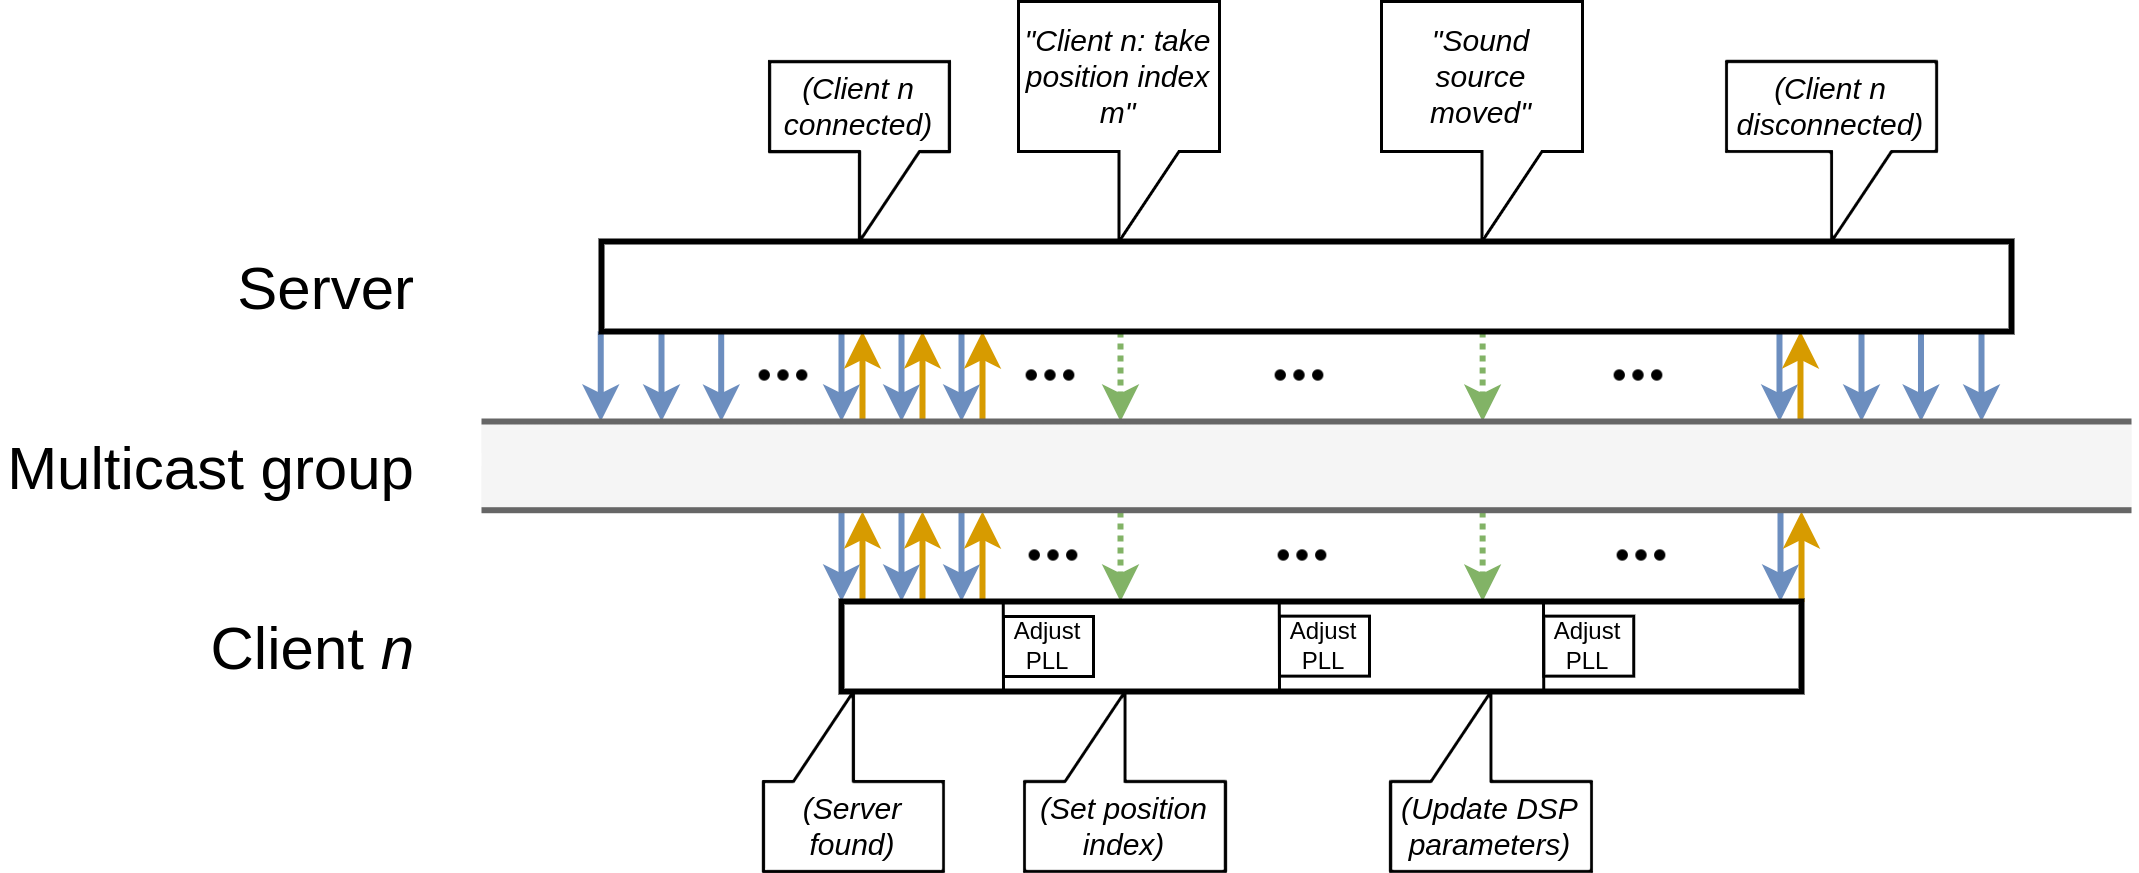
\includegraphics[width=\textwidth]{figures/timeline}
    \caption{Example timeline of client-server interaction. Blue arrows
    indicate audio data being sent from the server to the multicast group;
    orange arrows indicate audio data being sent from the client back to the
    multicast group;
    green arrows represent control data.}
    \label{fig:timeline}
\end{figure}

\subsubsection{Synchronicity with the Server}\label{subsubsec:client-sync}

Due to the influence of clock drift and transmission jitter, and since the
clients constitute a distributed system, with no direct knowledge of each other
and no authoritative source of time, their third task posed, without doubt,
the greatest challenge.

A two-pronged strategy was developed for addressing server-client and
inter-client timing discrepancies:

\paragraph{Jitter Compensation}
Similar to the approach taken in prior
work~\citep{rushton_microcontroller-based_2023}, clients monitored the difference
between the write and read positions to their intermediate audio buffer,
using a delay-locked loop to keep this difference within an interval of one
audio buffer.
This was achieved by way of setting thresholds for the read-write difference,
and adjusting the read-position increment if it fell beyond those thresholds;
increasing the increment if the difference exceeded the high threshold;
decreasing it should the difference fall short of the low threshold.
This in turn entailed employing a fractional read-position, and interpolating
around the read-position to achieve an appropriate sample value; essentially
a form of adaptive resampling.
For this purpose a cubic Lagrange interpolator was used; sample values for the
interpolator were converted from their 16-bit signed integer representation
to floating point numbers, interpolation conducted, and the resulting value
rounded to the nearest integer for output.

\paragraph{Clock Drift Compensation}
In the absence of an authoritative source of time, clients were set up to infer
the difference in rate between their own internal clock and that of the server
by comparing the rate of packet reception from the network to their internal
audio interrupt rate.
This was achieved by taking the ratio, over thirty-second intervals, of
packets written from the network to the intermediate buffer to blocks read
from the intermediate buffer for audio output.
This ratio was then used to calculate appropriate divisors to apply to the
\qty{24}{\MHz} master clock generated by a crystal oscillator on the Teensy,
adjusting the audio clock's phase locked ltheoop (PLL) to produce an adjusted audio
sampling rate.
The aim of this approach was to minimise reliance on the adaptive resampler
described above, and ultimately encourage all clients to run at the same audio
rate as the server.

\subsubsection{An Unexpected Source of Jitter}

Jitter does not arise solely during the journey from machine to machine across
a network.
It was found that, using the general purpose computer's default audio host
(ALSA), the timing of iterations of JUCE's audio processing loop, and thus
signals to \texttt{NetAudioServer}'s sender thread, was very uneven, i.e.\
subject to a high degree of jitter.
Though the average rate of execution was commensurate with the selected sample
rate and audio buffer size, individual audio buffer intervals differed, in
microsecond terms, by up to an order of magnitude.
This inconsistent audio timing was sufficient to cause transmission jitter that
overwhelmed the client-side strategy for jitter compensation.
The result was persistent audible distortion due to rapid fluctuations in the
client's audio buffer read-position increment.

Switching from ALSA to JACK as the audio host resolved this issue, but since
JACK \textit{uses} ALSA as its underlying audio host, this phenomenon was
difficult to account for.
A detailed description lies beyond the scope of this report, but
essentially JACK uses \textit{direct memory access} to map the underlying audio
device into memory,\footnote{
    Credit goes to Stéphane Letz, a prominent contributor to the JACK project,
    for providing this bit of context.
} and seemingly does so in a more effective manner than the driver
for the sound card on the development machine.
It is not known at the time of writing whether using ALSA with an external audio
interface (a potential barrier to entry) would have improved the situation.

This incident serves to illustrate that, beyond the concerns associated
with effective software design, a system such as the one described here, for
which the timing of operations is critical, is subject to the whims of a variety
of supporting hardware and software systems \textemdash{} things that in a more
conventional audio system can, to a greater degree, be taken for granted.
The topic of whether to attempt to compensate for this manner of phenomenon in
software or impose strict requirements on a future end-user in terms the audio
host they should use (something that would almost certainly vary with the user's
operating system), remains one for future research.

%\subsubsection{A Note on the Client-Server Dichotomy}\label{subsubsec:client-server}
%
%In principle, there is no meaningful impediment to the so-called
%clients acting as servers in their own right; a change of port number is all
%that would be required for each client to receive traffic from (and send
%traffic to) not just the server, but also from (and to) all other clients.
%Consequently, in code for both the server and clients, networked audio entities
%in the system are referred to as \textit{peers} (see, e.g.
%\figref{fig:plugin-interface}).
%In practice, and for the particular application
%\textemdash{} distributed spatial audio \textemdash{}
%considered here, receiving UDP packets from sources other than the designated
%server is not only unnecessary, but also manifestly inefficient.
%With Chafe et al.'s \textit{Internet Acoustics} work in mind, it is likely that
%there are some very interesting uses for a \textit{promiscuous} network
%of audio peers, but, for now, such applications lie beyond the scope of this
%work.

% \missingfigure{Diagram of signal format conversion, transmission, reception,
%     and re-conversion, i.e. UDP packets, sample buffers.}

\subsection{The Audio Spatialisation Algorithm}\label{subsec:wfs-algorithm}

With some modifications, e.g.\ the possibility to specify speaker spacing
parametrically, the WFS algorithm
from~\citep{rushton_microcontroller-based_2023} was reused.
This algorithm was written in Faust and compiled to
a C++ class compatible with the Teensy audio library via Faust's
\texttt{faust2teensy} utility.
Hardware modules were connected to a general purpose computer via a USB hub
and the \texttt{tycmd} utility from the TyTools suite (see
\secref{subsec:hardware-platforms}) was used to ensure that all modules were
programmed with the same instructions.

Implementing Huygens' principle in a digital audio system entails applying
delays to an audio signal representing a virtual sound source based on the
intended position of that sound source with respect to the secondary point
sources.
To limit the computational burden placed on the hardware modules, specifically
with regard to memory, the length of the delay lines was reduced by discarding
the longitudinal component of $r_k$, leaving only the relative inter-speaker
delay.
Additionally, a simplified WFS prefilter was employed, using the distance
from each virtual sound source to each secondary point source to an inverse
square law mapping for frequency-independent amplitude loss to the medium of
propagation, and the cutoff of a two-pole lowpass filter.
Adopting a modified version of equation~\eqref{eq:driving-function}, the
driving function becomes:
\begin{equation}
    \label{eq:simple-driving-function}
    d_k(\bfx,t) = f(t, r_k) \ast \delta\left(t - \frac{r_k-y_k}{c}\right).
\end{equation}
In implementation, the prefilter was tuned by ear using Faust's
\texttt{fi.lowpass} function\footnote{
    \url{https://faustlibraries.grame.fr/libs/filters/\#filowpass}
};
a thorough treatment of the simulation of distance effects in WFS stands as a
topic for future work.

\subsubsection{Modularity and Maximum Delay}

The reduction in the maximum delay length represented by the subtraction of
the longitudinal distance component in
equation~\eqref{eq:simple-driving-function} is essential for the viability of
the system.
As capable a platform as Teensy 4.1 is, as described in
\secref{subsec:hardware-platforms}, it is limited in terms of memory.
This in turn places limits on the lengths of delay lines that it can compute,
a matter exacerbated if there are many such delays to consider, such as in the
case of a WFS implementation with numerous virtual sound sources.
Each hardware module must compute two delay lines for each virtual source, one
for each of its output channels, the maximum length of which (depending on
the position of a given module in the speaker array) corresponds, after removal
of the longitudinal component, of the width of the speaker array.
It was observed that, for eight virtual sources and eight hardware modules,
the maximum speaker spacing permissible lay at around \qty{.4}{\m},
corresponding with a speaker array of maximum width 15 $\times$ 0.4 =
\qty{6}{\m}, equating to a maximum delay of $\sim$\qty{17}{\ms} or
approximately 795 samples at a sampling rate of \qty{44.1}{\kHz}.
The matter has not been rigorously tested, but nonetheless the presumption is
that this places significant limits on the modularity of the system.
Teensy's memory capacity can be extended by attaching up to two inexpensive
PSRAM chips for a further \qty{16}{\mega\byte} of memory.
These chips must be soldered onto the Teensy board, however, and the suitability
of such additional memory for rapid access, such as is required in an audio DSP
algorithm, remains to be investigated.

\subsubsection{Controlling the WFS Algorithm}

Parameter values are delivered to the Faust algorithm in the form of OSC
messages.
OSC control data, describing virtual sound source positions, speaker spacing,
and informing clients of their position in the speaker array, is bundled into
UDP packets and delivered by the server to the multicast group for all clients
to consume.

\codeinputlisting[float=h]
{text}
{listings/control-data-packet.txt}
{Network capture: ethernet frame containing a UDP control data packet}
{control-data-packet}

\lstref{listing:control-data-packet} demonstrates an example control data
packet, an OSC bundle containing one message.
This message has address \texttt{/source/0/x}, indicating that it refers to the
$x$-coordinate of the zeroth sound source, providing a value in the form of a
big-endian 32-bit floating point number, \texttt{0x3d1b5fa2}, approximately
\numDec{0.038}.

\subsection{System Overview}\label{subsec:system-overview}

\begin{figure}[ht]
    \centering
    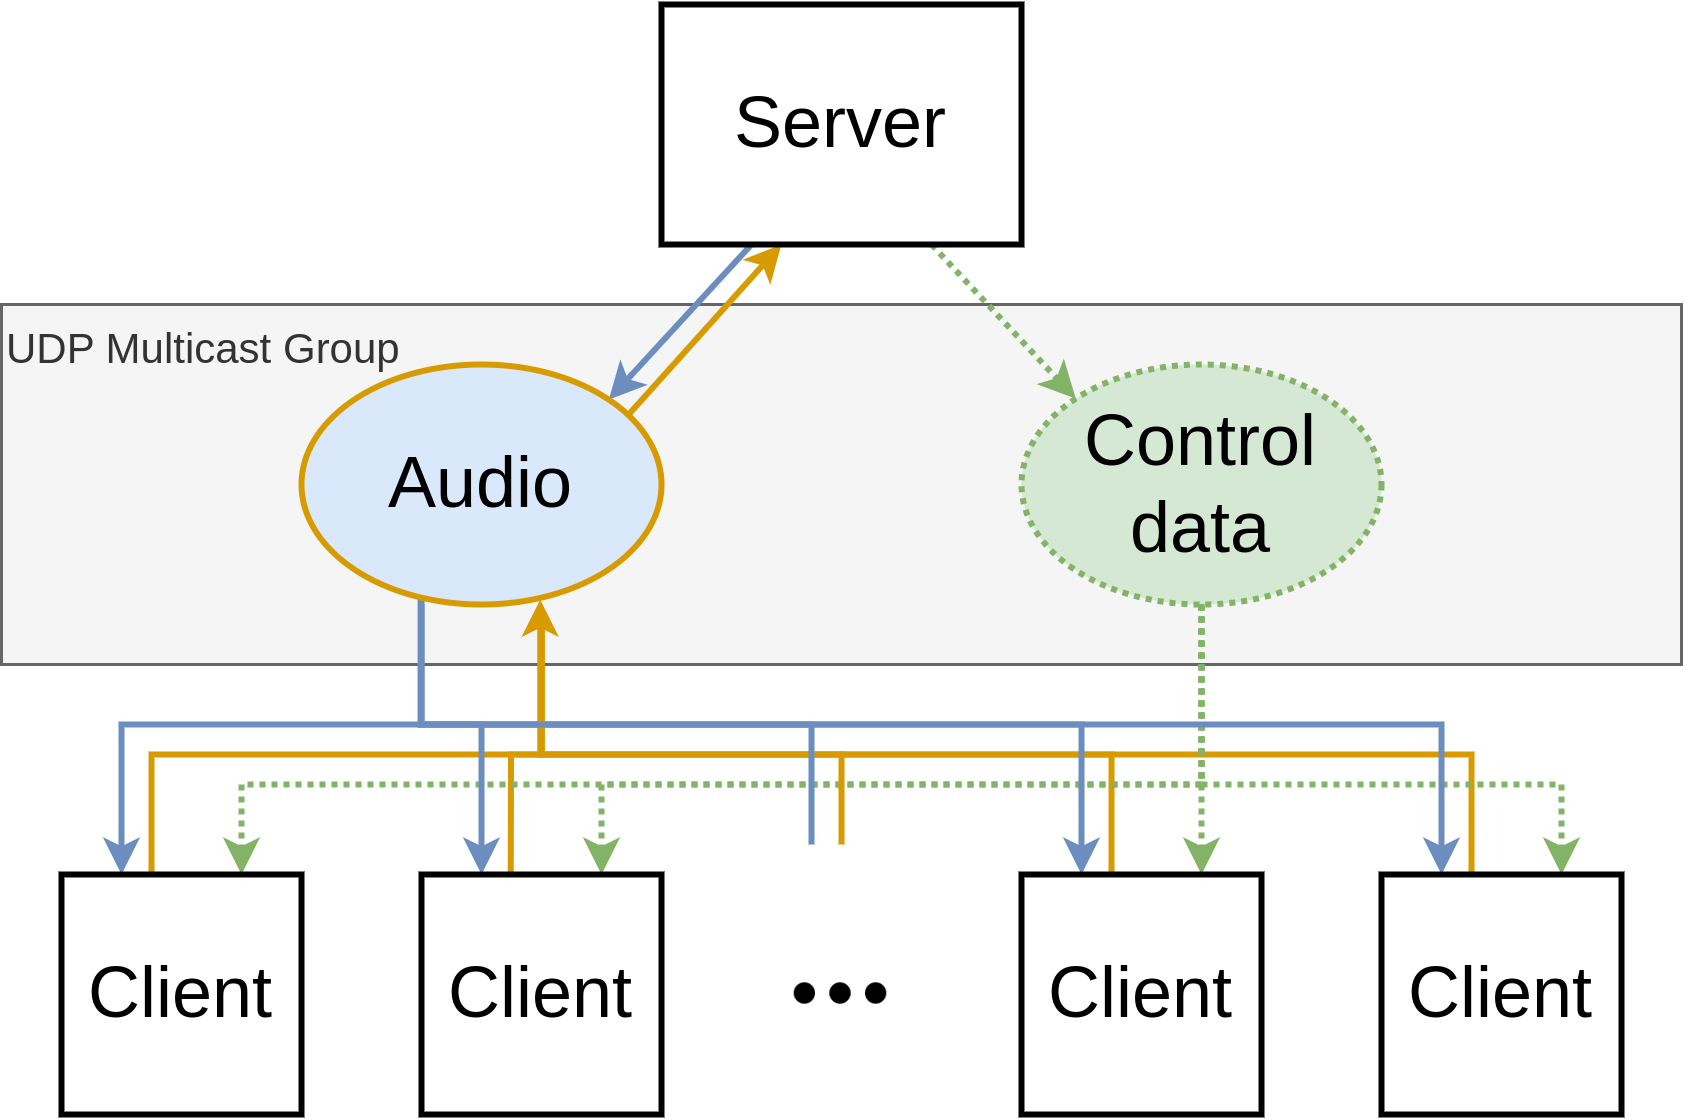
\includegraphics[width=.75\textwidth]{figures/multicast}
    \caption{Architecture of the networked audio system.
    The server sends audio and control data to a UDP multicast group on
    distinct port numbers; clients listen for this data, and send an audio
    stream back to the multicast group with which the server can register
    their presence on the network.}
    \label{fig:architecture}
\end{figure}

The proposed system being composed of multiple hardware and software components,
it is worthwhile to summarise the nature of these components and the
interactions between them.

\subsubsection{Hardware Setup}

The network audio server runs on a general purpose computer.
During the development and testing of this project, that computer was an ASUS
G513R Notebook PC, with an AMD Ryzen 7 6800H processor with a clock
speed of \qty{3.2}{\GHz}.
For the majority of development, the computer's internal sound card was used;
for testing and evaluation, it was connected to a Steinberg UR44C USB audio
interface in the hope that this would provide better reliability in terms of
audio interrupt timing.

The computer was connected via CAT6 ethernet cable to an eight-port ethernet
switch (D-Link DGS-108GL).
For evaluation, and to support a total of eight network audio clients, this
switch was daisy-chained to an additional switch (D-Link DES-1008D).
Teensy 4.1 hardware modules, assembled as per \figref{fig:teensy}, were
connected via CAT6 ethernet cables to available ports on the ethernet switches.
Hardware modules were powered by a combination of a seven-port USB hub, plus,
for the eighth module, a USB mains socket.
The two audio outputs of each hardware module were connected to M-Audio BX5
speakers.

\subsubsection{Software System}\label{subsubsec:software-system}

\begin{figure}[ht]
    \centering
    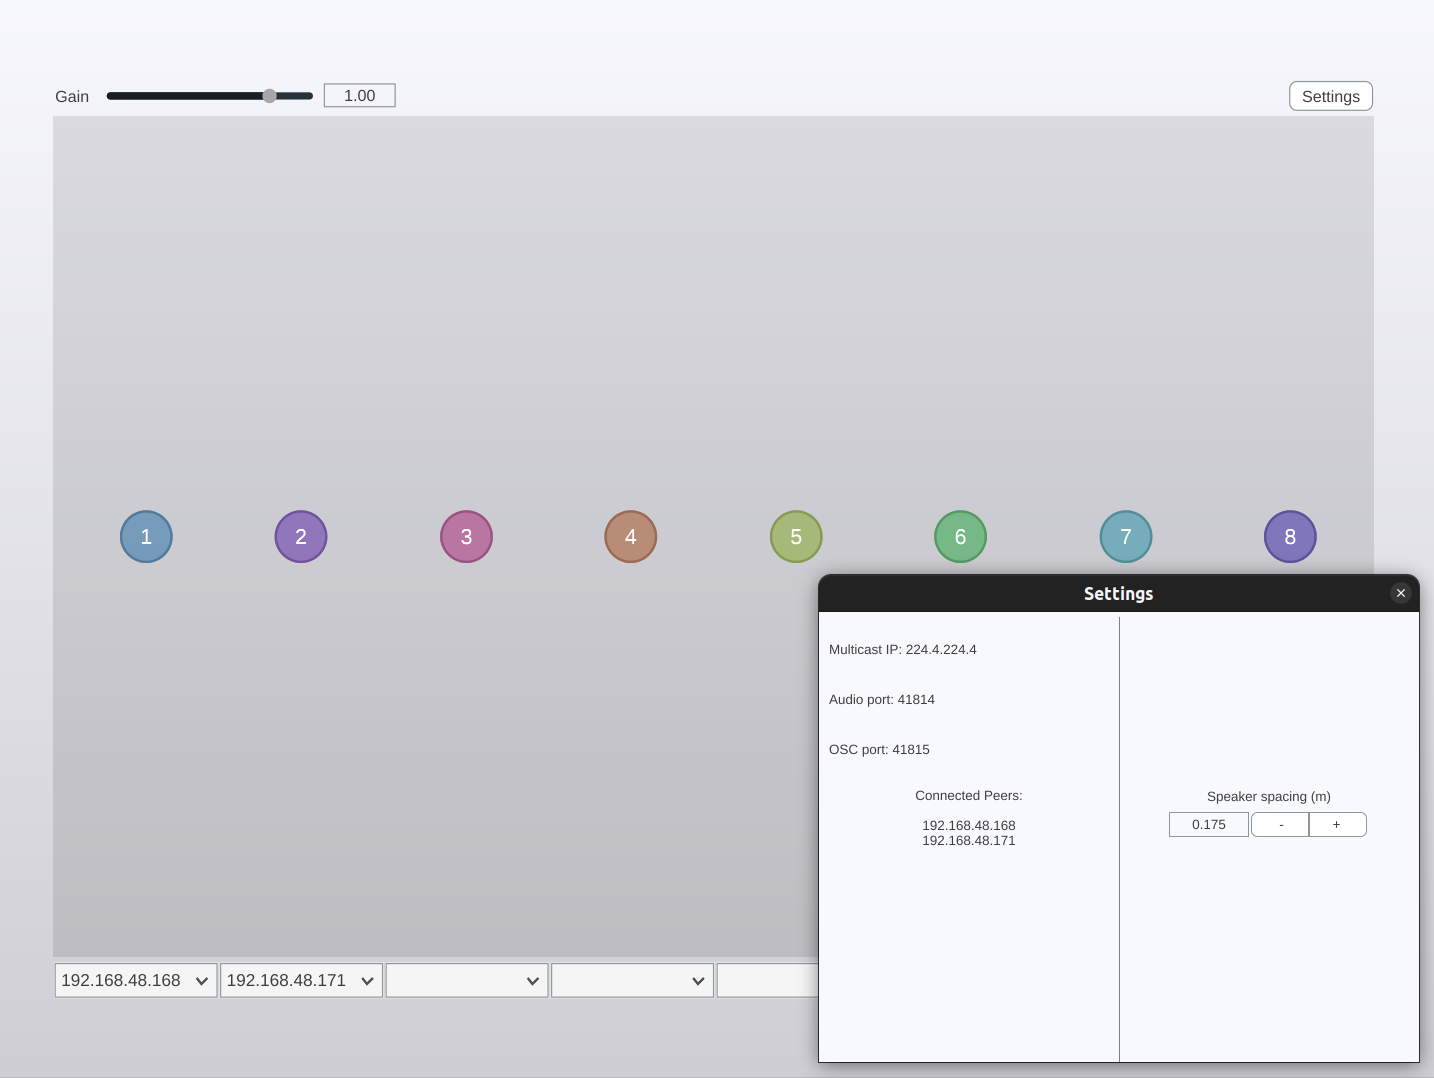
\includegraphics[width=\textwidth]{figures/plugin}
    \caption{
        User interface for the WFS controller DAW plugin, with modal
        settings window visible.
        The interface consists of an X/Y control surface, with eight nodes
        representing the locations of sound sources in a virtual sound field.
        Dropdown menus at the bottom of the interface correspond with hardware
        module positions in the loudspeaker array.
        The settings window facilitates specifying the speaker spacing, and
        shows a list of connected network peers.
    }
    \label{fig:plugin-interface}
\end{figure}

Server-side, the software system consists of a VST plugin running in Reaper
digital audio workstation software\footnote{\url{https://reaper.fm/}}.
The plugin comprises the networked audio server, receiving monophonic audio
sources in the form of audio or instrument tracks in the DAW, plus a control
data server, commanded either by parameter automation via the DAW, or manually
via a graphical user interface (see \figref{fig:plugin-interface}).
The audio and control data servers send streams of UDP packets to a UDP
multicast group.

Client-side software connects to the multicast group and reads UDP packets
containing audio and control data from the server.
These streams are delivered to the Faust-based WFS algorithm, with audio
streams processed according to the control parameters of virtual sound source
positions and speaker spacing.
The WFS algorithm produces driving signals for each of the two output channels
of the hardware module on which it is running.
Additionally, the client-side networked audio client returns a stream of audio
data to the multicast group, to be consumed by the server.

A diagram of the fundamental system architecture is shown in
\figref{fig:architecture}.
Code for the server and client software components can be found at
\url{https://github.com/hatchjaw/netjuce} and
\url{https://github.com/hatchjaw/netjuce-teensy} respectively.\todo[inline]{
    Document code repos.
}

% \begin{figure}[ht]
%     \centering
%     \includegraphics[width=\textwidth]{figures/system-overview.jpg}
%     \caption{System overview.}
%     \label{fig:system-overview}
% \end{figure}
